\documentclass[10pt]{article}
\usepackage[a4paper,margin=18mm]{geometry}
\usepackage[T1]{fontenc}\usepackage{lmodern}
\usepackage{amsmath,amssymb,booktabs,array,enumitem}
\usepackage{tikz}\usetikzlibrary{shapes.gates.logic.US,positioning,arrows.meta,patterns,calc}
\usepackage[hidelinks]{hyperref}
\setlength{\parindent}{0pt}\setlength{\parskip}{4pt}\setlength{\emergencystretch}{2em}
\newcommand{\mos}[4]{\begin{scope}[shift={(#1,#2)}]
\draw(0,.24)--(0,-.24);\draw(0,.2)--(.25,.2)--(.25,.5);\draw(0,-.2)--(.25,-.2)--(.25,-.5);
\draw(-.16,.23)--(-.16,-.23);
\ifnum#4=1\draw(-.26,0)circle(.06);\draw(-.75,0)--(-.32,0);\else\draw(-.75,0)--(-.16,0);\fi
\node[anchor=east,font=\scriptsize]at(-.76,0){$#3$};\end{scope}}
\newcommand{\gnd}[2]{\draw(#1,#2)--(#1,{#2-.12});\draw({#1-.17},{#2-.12})--({#1+.17},{#2-.12});\draw({#1-.11},{#2-.2})--({#1+.11},{#2-.2});}
\newcommand{\rail}[3]{\draw(#1,#2)--(#1,{#2+.14});\node[above,font=\scriptsize]at(#1,{#2+.14}){$#3$};}
\begin{document}
\begin{center}{\Large 2016 Final: Independently Derived Solutions}\end{center}
\textbf{Scope and provenance.} All original Q1--Q8 are complete, with printed total 120 points. The paper is filed under the 2021 folder, but its original footer explicitly says Fall 2016. No matching student answer was located. The supplied original controls equations, clock polarity and layout contacts; no answer has been reconstructed from another year's student work.

Width factors below multiply the source's $2\,\mu m/0.18\,\mu m$ device. Gate capacitance scales with width, NMOS ON resistance is $R/s_n$, and equal-width PMOS resistance is $2R/s_p$ where the question gives $\mu_n=2\mu_p$. Timing uses the source's elementary ON-resistor and ideal-clock models. Standard pMOS bodies connect to $V_{DD}$ and nMOS bodies to GND. No process-model simulation or unstated numeric device parameter is used.

\section*{Question 1: NP domino and the sizing ambiguity}
For $CLK=0,\overline{CLK}=1$, P1 precharges $X$ high, N2 disables the n-logic path, and the fixed output NMOS resets Out low. For $CLK=1,\overline{CLK}=0$, N1/N2 discharge $X$ if In=1; that falling $X$ enables P3 while P2 is on, charging Out high. With In=0, $X$ retains its precharged high and Out retains zero. Thus the valid evaluation result is
\[\boxed{Out=In,\qquad X=\overline{In}.}\]
The input must obey the usual n-dynamic evaluation monotonicity/stability rule; a late return from 1 to 0 cannot recharge $X$ before the next precharge. The two clock signals have nonoverlapping asserted phases as stated.

Let $N1=N2=n$, $P1=p_1$ and $P2=P3=p$. Only the gate of P3 loads $X$, so $C_X=pC$; Out has the fixed $4C$ load. The four RC transition estimates are
\[t_{rX}=\frac{2p}{p_1}RC,\quad t_{fX}=\frac{2p}{n}RC,\qquad
t_{rOut}=\frac{16}{p}RC,\quad t_{fOut}=4RC.\]
\textbf{Literal per-node balance.} Requiring equal rise/fall time at each node gives $p_1=n$ and $p=4$, while $n$ remains free. Reset transitions occur in parallel, but evaluation must discharge $X$ and then charge Out. A 50\% duty cycle therefore requires
\[\boxed{T_{min}(n)=2\left(\frac8n+4\right)RC=\left(8+\frac{16}{n}\right)RC.}\]
The required widths are $W_{N1}=W_{N2}=W_{P1}=2n\,\mu m$ and $W_{P2}=W_{P3}=8\,\mu m$, all at $0.18\,\mu m$ length. There is no finite globally optimal $n$ without a width, input/clock load or power bound: the period approaches $8RC$ as $n\to\infty$.

\textbf{An additional common-time design.} If ``$t_r=t_f$ for the nodes X and Out'' is additionally taken to mean the \emph{same} transition time for both nodes, that extra equation is $8/n=4$. Then $n=2$, giving N1/N2/P1=$4\,\mu m/0.18\,\mu m$, P2/P3=$8\,\mu m/0.18\,\mu m$, four transition times $4RC$, and $T_{min}=16RC$. This is a feasible common-time design, not a unique consequence of per-node equality alone.

The clock gate loads are P1+N2 on CLK and P2+the fixed output NMOS on $\overline{CLK}$. One charging event per clock cycle gives
\[\boxed{P_{clk}=[2n+5]fCV_{dd}^{2}.}\]
At the explicitly added common-time choice $n=2$, this becomes $9fCV_{dd}^{2}$. Clock-driver internal losses and unspecified wiring are outside the stated model.
\newpage
\section*{Question 2: what the waveform determines}
Let $V_H$ and $V_L$ be the rising-input and falling-input trip voltages. In the source's square-law turn-on balance, neglect body effect and use its fixed $0.6\,V$ thresholds.

Before a rising-input trip, $V_{out}=V_{DD}$ turns N3 on. N2 starts conducting at $V_a=V_H-V_{tn}$. Current balance between N1 and N3 then gives
\[\frac{\beta_{N1}}2(V_H-V_{tn})^2
=\frac{\beta_{N3}}2(V_{DD}-V_H)^2,
\qquad\boxed{\frac{\beta_{N1}}{\beta_{N3}}=
\left(\frac{1.8-V_H}{V_H-0.6}\right)^2.}\]
Before a falling-input trip, $V_{out}=0$ turns P3 on. P2 starts conducting at $V_b=V_L+|V_{tp}|$, giving
\[\frac{\beta_{P1}}2(V_{DD}-V_L-|V_{tp}|)^2
=\frac{\beta_{P3}}2V_L^2,
\qquad\boxed{\frac{\beta_{P1}}{\beta_{P3}}=
\left(\frac{V_L}{1.2-V_L}\right)^2.}\]
The shown output stays low through the first downward excursion to $0.6\,V$ and its rebound, then rises when the input falls through approximately $0.6\,V$ at $t_1$. Taking the marked lower trip as $V_L=0.6\,V$ gives $\beta_{P1}/\beta_{P3}=1$ in this model.

\textbf{The upper ratio is not numerically determined.} The $1.2\,V$ mark accompanies the input-noise rebound, which stays at or below that level while the output is already low. There is no rising-input transition from the high-output state to identify $V_H$. A rebound while the output is low cannot measure the rising-input trip. Hence the waveform does not justify setting $V_H=1.2\,V$ or concluding $\beta_{N1}/\beta_{N3}=1$. For ordinary hysteresis with the inferred lower trip, the admissible upper trip satisfies $0.6<V_H<1.8\,V$; the boxed formula supplies the corresponding family. An actual upper trip or another sizing constraint is needed for a scalar answer.

\textbf{Short-circuit power.} An unconditional higher-or-smaller comparison is not fixed by the supplied ratios and waveform: absolute widths/current strengths and input time scales are missing. The feedback circuit introduces direct contention paths $V_{DD}\to N3\to N1\to GND$ while the output is high, and $V_{DD}\to P1\to P3\to GND$ while it is low. A slowly moving/noisy input can keep one of these paths conducting even while the output is held at a rail, permitting increased DC contention compared with the feedback-free circuit. Regeneration also sharpens the output transition and can change the main-stack current interval. Consequently, the added paths explain a possible power increase, but the schematic alone does not prove a universal total-power ordering. No numeric current or energy is invented.
\newpage
\section*{Question 3: clock-capacitance constraint and keeper}
Reading the original n-network, N1 is parallel with an upper subnetwork N2 in parallel with N4--N5, followed by N3 in parallel with N6. N7 is the common clock footer. The complete conducting paths are
\[N1--N7;\quad N2--N3--N7;\quad N2--N6--N7;\quad
N4--N5--N3--N7;\quad N4--N5--N6--N7.\]
Only P1 and N7 are clock loads, so $s_{P1}+s_{N7}=9$. The source gives no unique minimum-area or delay target; it permits a sizing family. Let $p=s_{P1}$, $s_{N7}=9-p$ and
\[\Delta=\frac2p-\frac1{9-p}>0,\qquad 0<p<6.\]
Choose
\[s_{N1}=\frac1\Delta,\quad s_{N2}=s_{N3}=s_{N6}=\frac2\Delta,
\quad s_{N4}=s_{N5}=\frac4\Delta.\]
Each isolated conducting path has resistance $2R/p$, matching P1's charging resistance. Thus both worst-case node-X transitions use $(2R/p)C_X$. Parallel enabled branches can make a fall faster; worst-case balance does not mean all input combinations have an identical discharge time.

A simple exact design chooses $p=3$:
\begin{center}\begin{tabular}{lrrrrrrrr}\toprule
Device&P1&N1&N2&N3&N4&N5&N6&N7\\\midrule
Width factor&3&2&4&4&8&8&4&6\\
Width ($\mu m$)&6&4&8&8&16&16&8&12\\\bottomrule
\end{tabular}\end{center}
All lengths are $0.18\,\mu m$. P1+N7 gate capacitance is $9C$, so $P_{CLK}=9fCV_{dd}^{2}$. Every listed isolated path has resistance $2R/3$. The inverter input capacitance $C_X$ is not numerically specified because P2/N8 sizes are not given; it cancels in the rise/fall comparison.

For retention, add a \emph{weak} pMOS keeper from $V_{DD}$ to X with its gate connected to the existing static inverter output Y:
\begin{center}\begin{tikzpicture}[x=.92cm,y=.92cm,font=\scriptsize]
\mos{0.0}{0.0}{Y}{1}
\node[right]at(0.43,0.0){$\mathrm{Pkeeper}$};
\node[above]at(0.25,0.52){$V_{DD}$};
\node[below]at(0.25,-0.52){$X$};
\end{tikzpicture}\end{center}
When X=1, Y=0 turns the keeper on and replenishes leakage. When the pull-down begins a legitimate evaluation discharge, it must overcome the keeper; after Y rises, the keeper turns off. The keeper must be weak enough for evaluation and strong enough for retention. Its gate is not driven by CLK, so it does not alter the stipulated clock gate-capacitance total. No numeric keeper width follows from the supplied leakage-free sizing model.
\newpage
\section*{Question 4: exact physical MOS extraction}
Each layout has six diffusion-crossing gate columns per row, giving 12 physical MOS. All internal node labels below are added for readable electrical connections. Equal terminal names are wired together.
\textbf{(a) Literal twelve-device schematic:}
\begin{center}\begin{tikzpicture}[x=.92cm,y=.92cm,font=\scriptsize]
\mos{0.0}{0.0}{Y}{1}
\node[right]at(0.43,0.0){$\mathrm{P1}$};
\node[above]at(0.25,0.52){$V_{DD}$};
\node[below]at(0.25,-0.52){$u$};
\mos{3.9}{0.0}{Y}{0}
\node[right]at(4.33,0.0){$\mathrm{N1}$};
\node[above]at(4.15,0.52){$GND$};
\node[below]at(4.15,-0.52){$u$};
\mos{7.8}{0.0}{C}{1}
\node[right]at(8.23,0.0){$\mathrm{P2}$};
\node[above]at(8.05,0.52){$u$};
\node[below]at(8.05,-0.52){$v$};
\mos{11.7}{0.0}{\bar C}{0}
\node[right]at(12.129999999999999,0.0){$\mathrm{N2}$};
\node[above]at(11.95,0.52){$u$};
\node[below]at(11.95,-0.52){$v$};
\mos{0.0}{-2.2}{\bar C}{1}
\node[right]at(0.43,-2.2){$\mathrm{P3}$};
\node[above]at(0.25,-1.6800000000000002){$v$};
\node[below]at(0.25,-2.72){$r$};
\mos{3.9}{-2.2}{C}{0}
\node[right]at(4.33,-2.2){$\mathrm{N3}$};
\node[above]at(4.15,-1.6800000000000002){$v$};
\node[below]at(4.15,-2.72){$r$};
\mos{7.8}{-2.2}{X}{1}
\node[right]at(8.23,-2.2){$\mathrm{P4}$};
\node[above]at(8.05,-1.6800000000000002){$r$};
\node[below]at(8.05,-2.72){$V_{DD}$};
\mos{11.7}{-2.2}{X}{0}
\node[right]at(12.129999999999999,-2.2){$\mathrm{N4}$};
\node[above]at(11.95,-1.6800000000000002){$r$};
\node[below]at(11.95,-2.72){$GND$};
\mos{0.0}{-4.4}{v}{1}
\node[right]at(0.43,-4.4){$\mathrm{P5}$};
\node[above]at(0.25,-3.8800000000000003){$V_{DD}$};
\node[below]at(0.25,-4.92){$X$};
\mos{3.9}{-4.4}{v}{0}
\node[right]at(4.33,-4.4){$\mathrm{N5}$};
\node[above]at(4.15,-3.8800000000000003){$GND$};
\node[below]at(4.15,-4.92){$X$};
\mos{7.8}{-4.4}{X}{1}
\node[right]at(8.23,-4.4){$\mathrm{P6}$};
\node[above]at(8.05,-3.8800000000000003){$X$};
\node[below]at(8.05,-4.92){$V_{DD}$};
\mos{11.7}{-4.4}{X}{0}
\node[right]at(12.129999999999999,-4.4){$\mathrm{N6}$};
\node[above]at(11.95,-3.8800000000000003){$X$};
\node[below]at(11.95,-4.92){$GND$};
\end{tikzpicture}\end{center}
The input inverter is Y$\to u$. The two input/feedback switches are TG2: $u\leftrightarrow v$, p gate C/n gate $\bar C$, and TG3: $v\leftrightarrow r$, p gate $\bar C$/n gate C. Column 4 is X$\to r$; column 5 is $v\to X$. The upper/lower bent poly at column 5 connects both TG2 drain regions to v. The middle C metal strip contacts the upper column-2 gate and lower column-3 gate; its crossing with the bent $\bar C$ poly has no contact.

\textbf{Important literal source feature:} column 6 has \emph{both gate and joined drains connected to X}, with its other p/n terminals at $V_{DD}$/GND. The X horizontal M1 crosses the vertical shared column-5/6 drain strip, and no break is visible. This is a self-connected CMOS pair; it is retained in the extraction. At an assumed binary X=0 its pMOS pulls upward, and at X=1 its nMOS pulls downward. A clean, unconditional digital latch behavior cannot be claimed from this literal graph. The question asks extraction; silently splitting the wire or replacing the last pair by an output inverter would change the original.

\textbf{(b) Literal twelve-device schematic:}
\begin{center}\begin{tikzpicture}[x=.92cm,y=.92cm,font=\scriptsize]
\mos{0.0}{0.0}{a}{1}
\node[right]at(0.43,0.0){$\mathrm{P1}$};
\node[above]at(0.25,0.52){$V_{DD}$};
\node[below]at(0.25,-0.52){$u$};
\mos{3.9}{0.0}{a}{0}
\node[right]at(4.33,0.0){$\mathrm{N1}$};
\node[above]at(4.15,0.52){$GND$};
\node[below]at(4.15,-0.52){$u$};
\mos{7.8}{0.0}{V_{DD}}{1}
\node[right]at(8.23,0.0){$\mathrm{P2}$};
\node[above]at(8.05,0.52){$u$};
\node[below]at(8.05,-0.52){$V_{DD}$};
\mos{11.7}{0.0}{GND}{0}
\node[right]at(12.129999999999999,0.0){$\mathrm{N2}$};
\node[above]at(11.95,0.52){$u$};
\node[below]at(11.95,-0.52){$GND$};
\mos{0.0}{-2.2}{u}{1}
\node[right]at(0.43,-2.2){$\mathrm{P3}$};
\node[above]at(0.25,-1.6800000000000002){$V_{DD}$};
\node[below]at(0.25,-2.72){$s1$};
\mos{3.9}{-2.2}{u}{0}
\node[right]at(4.33,-2.2){$\mathrm{N3}$};
\node[above]at(4.15,-1.6800000000000002){$GND$};
\node[below]at(4.15,-2.72){$Z$};
\mos{7.8}{-2.2}{b}{1}
\node[right]at(8.23,-2.2){$\mathrm{P4}$};
\node[above]at(8.05,-1.6800000000000002){$s1$};
\node[below]at(8.05,-2.72){$s2$};
\mos{11.7}{-2.2}{b}{0}
\node[right]at(12.129999999999999,-2.2){$\mathrm{N4}$};
\node[above]at(11.95,-1.6800000000000002){$Z$};
\node[below]at(11.95,-2.72){$GND$};
\mos{0.0}{-4.4}{c}{1}
\node[right]at(0.43,-4.4){$\mathrm{P5}$};
\node[above]at(0.25,-3.8800000000000003){$s2$};
\node[below]at(0.25,-4.92){$Z$};
\mos{3.9}{-4.4}{c}{0}
\node[right]at(4.33,-4.4){$\mathrm{N5}$};
\node[above]at(4.15,-3.8800000000000003){$GND$};
\node[below]at(4.15,-4.92){$Z$};
\mos{7.8}{-4.4}{V_{DD}}{1}
\node[right]at(8.23,-4.4){$\mathrm{P6}$};
\node[above]at(8.05,-3.8800000000000003){$Z$};
\node[below]at(8.05,-4.92){$fp$};
\mos{11.7}{-4.4}{GND}{0}
\node[right]at(12.129999999999999,-4.4){$\mathrm{N6}$};
\node[above]at(11.95,-3.8800000000000003){$Z$};
\node[below]at(11.95,-4.92){$fn$};
\end{tikzpicture}\end{center}
\newpage
\section*{Question 4(b), continued}
Column 1 generates $u=\bar a$. The horizontal metal to column 3 begins on the inverter's vertical \emph{drain} strip; a visible white gap separates it from the local a gate bridge. Thus column 3 is driven by u, not a. P3--P4--P5 form a series pull-up; N3, N4 and N5 are parallel pull-down branches. The separate floating end diffusions of column 6 are $f_p,f_n$. The complete result is
\[\boxed{Z=\overline{u+b+c}=a\bar b\bar c.}\]
P2/P6 gates tie to $V_{DD}$, and N2/N6 gates tie to GND: all four isolation MOS are OFF. The layout contains eight functional MOS plus these four OFF physical devices. The apparent top-rail contact above the P3/P4 gap is not bridged downward into that internal series node. The verifier checks the twelve-device switch graph and all eight input words, including the inverter that supplies u.

\section*{Question 5: setup, hold and signed skew}
Let $A=R1.Q$, $B=R2.Q$, $C=R3.Q$. Exact diagram connectivity is
\[U=B\oplus C,\quad V=A\oplus C,\quad W=\bar V,\quad Z=\overline{U+W},
\quad R5.D=Z\odot A,\quad R6.D=V,\quad R4.D=A.\]
The sole explicitly given wire delay is $0.1\,ns$ on R1$\to$R4. Since one delay per gate is given, the elementary analysis uses it for both maximum and minimum gate delay; it does not invent separate contamination delays.
\begin{center}\begin{tabular}{lll}\toprule
Launch/capture&Structural route&Data delay (ns)\\\midrule
R1/R4&wire&0.1\\
R1/R5&final XNOR directly&0.4\\
R1/R5&XOR, INV, NOR, XNOR&1.4\\
R1/R6&lower XOR&0.5\\
R2/R5&upper XOR, NOR, XNOR&1.2\\
R3/R5&upper XOR, NOR, XNOR&1.2\\
R3/R5&lower XOR, INV, NOR, XNOR&1.4\\
R3/R6&lower XOR&0.5\\\bottomrule
\end{tabular}\end{center}
Zero-skew hold requires $0.1+t_{data,min}\ge0.4\,ns$. Only R1$\to$R4 fails, with $-0.2\,ns$ hold slack. Add two inverters \emph{only on the R4 branch after the A fanout}. Its delay becomes $0.1+2(0.2)=0.5\,ns$, preserving polarity and giving $+0.2\,ns$ hold slack. Placing them before the fanout would also delay the critical path.
\begin{center}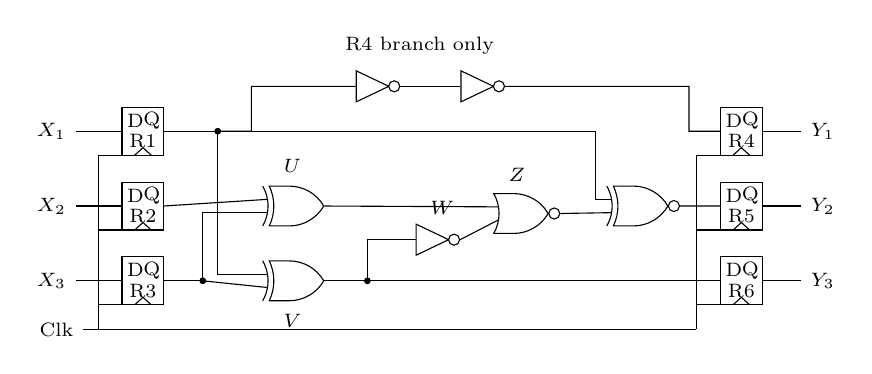
\begin{tikzpicture}[scale=.95,font=\scriptsize]
\draw(-0.28,1.68)rectangle(0.28,2.32);\node at(-0.1,2.14){D};\node at(0.12,2.14){Q};\node at(0,1.87){R1};
\draw(-0.11,1.68)--(0,1.78)--(0.11,1.68);
\draw(-0.28,2)--(-.9,2)node[left]{$X_{1}$};
\draw(-0.28,0.6799999999999999)rectangle(0.28,1.32);\node at(-0.1,1.1400000000000001){D};\node at(0.12,1.1400000000000001){Q};\node at(0,0.87){R2};
\draw(-0.11,0.6799999999999999)--(0,0.78)--(0.11,0.6799999999999999);
\draw(-0.28,1)--(-.9,1)node[left]{$X_{2}$};
\draw(-0.28,-0.32)rectangle(0.28,0.32);\node at(-0.1,0.14){D};\node at(0.12,0.14){Q};\node at(0,-0.13){R3};
\draw(-0.11,-0.32)--(0,-0.22)--(0.11,-0.32);
\draw(-0.28,0)--(-.9,0)node[left]{$X_{3}$};
\draw(7.72,1.68)rectangle(8.28,2.32);\node at(7.9,2.14){D};\node at(8.12,2.14){Q};\node at(8,1.87){R4};
\draw(7.89,1.68)--(8,1.78)--(8.11,1.68);
\draw(8.28,2)--(8.8,2)node[right]{$Y_{1}$};
\draw(7.72,0.6799999999999999)rectangle(8.28,1.32);\node at(7.9,1.1400000000000001){D};\node at(8.12,1.1400000000000001){Q};\node at(8,0.87){R5};
\draw(7.89,0.6799999999999999)--(8,0.78)--(8.11,0.6799999999999999);
\draw(8.28,1)--(8.8,1)node[right]{$Y_{2}$};
\draw(7.72,-0.32)rectangle(8.28,0.32);\node at(7.9,0.14){D};\node at(8.12,0.14){Q};\node at(8,-0.13){R6};
\draw(7.89,-0.32)--(8,-0.22)--(8.11,-0.32);
\draw(8.28,0)--(8.8,0)node[right]{$Y_{3}$};
\node[xor gate US,draw,logic gate inputs=nn](u)at(2,1){};\node[xor gate US,draw,logic gate inputs=nn](v)at(2,0){};
\node[not gate US,draw](w)at(3.8,.55){};\node[nor gate US,draw,logic gate inputs=nn](z)at(5.0,.9){};\node[xnor gate US,draw,logic gate inputs=nn](g)at(6.6,1){};
\draw(.28,1)--(u.input 1);\draw(.28,0)--(.8,0)|-(u.input 2);\draw(.8,0)--(v.input 2);\fill(.8,0)circle(1.3pt);
\draw(.28,2)--(1.0,2);\draw(1.0,2)|-(v.input 1);\fill(1.0,2)circle(1.3pt);
\draw(u.output)--(z.input 1);\draw(v.output)--(3,0);\draw(3,0)|-(w.input);\draw(w.output)--(z.input 2);\draw(z.output)--(g.input 2);
\draw(1.0,2)--(6.05,2)|-(g.input 1);\draw(g.output)--(7.72,1);\draw(3,0)--(7.72,0);\fill(3,0)circle(1.3pt);
\node[above]at(2,1.32){$U$};\node[below]at(2,-.32){$V$};\node[above]at(4,.75){$W$};\node[above]at(5,1.2){$Z$};
\node[not gate US,draw](d1)at(3,2.6){};\node[not gate US,draw](d2)at(4.4,2.6){};\draw(1,2)--(1.45,2)--(1.45,2.6)--(d1.input);\draw(d1.output)--(d2.input);\draw(d2.output)--(7.3,2.6)--(7.3,2)--(7.72,2);\node[above]at(3.7,2.9){R4 branch only};
\draw(-.8,-.65)--(7.4,-.65);\node[left]at(-.8,-.65){Clk};\draw(-.6,-.65)--(-.6,1.68);\draw(7.4,-.65)--(7.4,1.68);\draw(-.6,-.32)--(0,-.32);\draw(-.6,.68)--(0,.68);\draw(-.6,1.68)--(0,1.68);\draw(7.4,-.32)--(8,-.32);\draw(7.4,.68)--(8,.68);\draw(7.4,1.68)--(8,1.68);
\end{tikzpicture}\\Figure 5 with the zero-skew hold repair.\end{center}
\newpage
\section*{Question 5(b)--(c): attainable frequency}
The repaired longest path remains $1.4\,ns$. Therefore
\[\boxed{T_{min}=0.3+1.4+0.3=2.0\,ns,\qquad f_{max}=500\,MHz.}\]
The original has this setup bound but is invalid at any period because of hold. The long reconvergent R3 branch must be retained; an input transition can require the slow V/INV branch before both NOR inputs release.

The source gives an unsigned $0.5\,ns$ skew. Define $s=t_{capture}-t_{launch}$, with a common left/right clock-group offset. Then
\[T\ge2.0-s\;ns,\qquad t_{data,min}\ge0.3+s\;ns.\]
\begin{center}\begin{tabular}{lrrl}\toprule
Clock relation&s (ns)&Setup bound&Part-(a) hold result\\\midrule
Capture earlier&$-0.5$&400 MHz&all paths pass\\
Capture later&$+0.5$&666.7 MHz&four structural paths fail\\\bottomrule
\end{tabular}\end{center}
For positive skew, R1$\to$R4, the direct R1$\to$R5 branch, and R1/R3$\to$R6 have data delays below $0.8\,ns$. No clock-period reduction repairs hold. To make 666.7 MHz attainable, use four inverters \emph{total} on R4's branch ($0.9\,ns$), two on the dedicated $V\to R6$ branch after its fanout ($0.9\,ns$), and two on the dedicated $A\to$final-XNOR branch ($0.8\,ns$). These branch-only additions preserve every Boolean output and leave the $1.4\,ns$ longest path intact.

If skew means an unknown error bounded by $\pm0.5\,ns$, the safe combined result is \textbf{400 MHz with the stronger hold repair}: negative skew limits setup and positive skew limits hold. Quoting 666.7 MHz without its additional hold repair would be a setup-only answer, not a valid operating frequency.
\section*{Question 6: master setup and ratioed slave}
The source's master input TG is on at CLK=0; its feedback TG is on at CLK=1. The slave input TG is on at CLK=1, while feedback P2/N2 is always connected. Thus this is a positive-edge register. During low clock, Inv1's output B must acquire $\bar D$ before the edge. Its nominal setup interval is
\[\boxed{t_{setup}=t_{TG}+t_{Inv1}=0.1+0.2=0.3\,ns.}\]
Inv2 lies on the post-edge slave path and is not added to setup. This is the ideal forward-delay estimate, not a physical setup characterization requiring clock slew and node capacitances.

Let S be Inv2's input and use the source's $R_{TS}$ for the slave TG resistance. For old Q=0, P2 opposes a low write by pulling S up, while Inv1's N1 pulls down through the TG:
\[\frac{V_S}{V_{dd}}=\frac{R_{N1}+R_{TS}}{R_{P2}+R_{N1}+R_{TS}}<\frac12
\quad\Longleftrightarrow\quad\boxed{R_{P2}>R_{N1}+R_{TS}.}\]
For old Q=1, N2 opposes a high write while P1 supplies it through the TG:
\[\frac{V_S}{V_{dd}}=\frac{R_{N2}}{R_{P1}+R_{TS}+R_{N2}}>\frac12
\quad\Longleftrightarrow\quad\boxed{R_{N2}>R_{P1}+R_{TS}.}\]
The inequalities pair feedback P2 with driver N1, and feedback N2 with driver P1. Equality gives no regeneration margin. Weak feedback normally means smaller W/L, but no numerical widths follow from the given resistance model. After Q changes, the old opposing feedback device turns off and the new one assists retention.
\newpage
\section*{Question 7: three complete logic realizations}
The original overbar covers the entire product: $f=\overline{(A+BC)D}$. Define $h=(A+BC)D$ and $\bar h=\bar D+\bar A(\bar B+\bar C)$. The two complementary n-networks each use four MOS.

\textbf{Dynamic logic (6 MOS).} Precharge f with a CLK-gated pMOS, then evaluate through D in series with A in parallel with B--C, followed by a CLK footer. No output inverter is added because the requested f is the precharged inverted rail.
\begin{center}\begin{tikzpicture}[x=.92cm,y=.92cm,font=\scriptsize]
\mos{0.0}{0.0}{CLK}{1}
\node[right]at(0.43,0.0){$\mathrm{Ppre}$};
\node[above]at(0.25,0.52){$V_{DD}$};
\node[below]at(0.25,-0.52){$f$};
\mos{3.9}{0.0}{D}{0}
\node[right]at(4.33,0.0){$\mathrm{ND}$};
\node[above]at(4.15,0.52){$f$};
\node[below]at(4.15,-0.52){$h_0$};
\mos{7.8}{0.0}{A}{0}
\node[right]at(8.23,0.0){$\mathrm{NA}$};
\node[above]at(8.05,0.52){$h_0$};
\node[below]at(8.05,-0.52){$h_b$};
\mos{11.7}{0.0}{B}{0}
\node[right]at(12.129999999999999,0.0){$\mathrm{NB}$};
\node[above]at(11.95,0.52){$h_0$};
\node[below]at(11.95,-0.52){$h_1$};
\mos{0.0}{-2.2}{C}{0}
\node[right]at(0.43,-2.2){$\mathrm{NC}$};
\node[above]at(0.25,-1.6800000000000002){$h_1$};
\node[below]at(0.25,-2.72){$h_b$};
\mos{3.9}{-2.2}{CLK}{0}
\node[right]at(4.33,-2.2){$\mathrm{Nclk}$};
\node[above]at(4.15,-1.6800000000000002){$h_b$};
\node[below]at(4.15,-2.72){$GND$};
\end{tikzpicture}\end{center}
Inputs must be stable/monotonic during evaluation and retention must last until the next precharge. CLK=0 forces f=1; CLK=1 computes f. The truth/network verifier checks all sixteen input words.

\textbf{Fully differential logic (10-MOS core).} Use complementary n-networks under f and $g=\bar f=h$. Cross-couple the two pMOS loads to opposite full-swing output rails:
\begin{center}\begin{tikzpicture}[x=.92cm,y=.92cm,font=\scriptsize]
\mos{0.0}{0.0}{g}{1}
\node[right]at(0.43,0.0){$\mathrm{Pf}$};
\node[above]at(0.25,0.52){$V_{DD}$};
\node[below]at(0.25,-0.52){$f$};
\mos{3.9}{0.0}{f}{1}
\node[right]at(4.33,0.0){$\mathrm{Pg}$};
\node[above]at(4.15,0.52){$V_{DD}$};
\node[below]at(4.15,-0.52){$g$};
\mos{7.8}{0.0}{D}{0}
\node[right]at(8.23,0.0){$\mathrm{ND}$};
\node[above]at(8.05,0.52){$f$};
\node[below]at(8.05,-0.52){$p_0$};
\mos{11.7}{0.0}{A}{0}
\node[right]at(12.129999999999999,0.0){$\mathrm{NA}$};
\node[above]at(11.95,0.52){$p_0$};
\node[below]at(11.95,-0.52){$GND$};
\mos{0.0}{-2.2}{B}{0}
\node[right]at(0.43,-2.2){$\mathrm{NB}$};
\node[above]at(0.25,-1.6800000000000002){$p_0$};
\node[below]at(0.25,-2.72){$p_1$};
\mos{3.9}{-2.2}{C}{0}
\node[right]at(4.33,-2.2){$\mathrm{NC}$};
\node[above]at(4.15,-1.6800000000000002){$p_1$};
\node[below]at(4.15,-2.72){$GND$};
\mos{7.8}{-2.2}{\bar D}{0}
\node[right]at(8.23,-2.2){$\mathrm{Nd}$};
\node[above]at(8.05,-1.6800000000000002){$g$};
\node[below]at(8.05,-2.72){$GND$};
\mos{11.7}{-2.2}{\bar A}{0}
\node[right]at(12.129999999999999,-2.2){$\mathrm{Na}$};
\node[above]at(11.95,-1.6800000000000002){$g$};
\node[below]at(11.95,-2.72){$q_0$};
\mos{0.0}{-4.4}{\bar B}{0}
\node[right]at(0.43,-4.4){$\mathrm{Nb}$};
\node[above]at(0.25,-3.8800000000000003){$q_0$};
\node[below]at(0.25,-4.92){$GND$};
\mos{3.9}{-4.4}{\bar C}{0}
\node[right]at(4.33,-4.4){$\mathrm{Nc}$};
\node[above]at(4.15,-3.8800000000000003){$q_0$};
\node[below]at(4.15,-4.92){$GND$};
\end{tikzpicture}\end{center}
When h=1, the f network pulls f down and the pMOS on g restores g high; when h=0, the complementary network reverses these roles. Appropriate n/p strengths are needed during regeneration. Complemented inputs are generated explicitly on the next page.
\newpage
\section*{Question 7: differential split-level and input generators}
\textbf{DSL (12-MOS core).} The same complementary n-networks drive low-swing nodes p,q. Two reference-gated nMOS connect them to full-swing outputs f,g. The load on f is driven by \emph{opposite internal node q}, and the load on g by p, as in the lecturer's Chapter 6 slide 32:
\begin{center}\begin{tikzpicture}[x=.92cm,y=.92cm,font=\scriptsize]
\mos{0.0}{0.0}{q}{1}
\node[right]at(0.43,0.0){$\mathrm{Pf}$};
\node[above]at(0.25,0.52){$V_{DD}$};
\node[below]at(0.25,-0.52){$f$};
\mos{3.9}{0.0}{p}{1}
\node[right]at(4.33,0.0){$\mathrm{Pg}$};
\node[above]at(4.15,0.52){$V_{DD}$};
\node[below]at(4.15,-0.52){$g$};
\mos{7.8}{0.0}{V_{ref}}{0}
\node[right]at(8.23,0.0){$\mathrm{NrefF}$};
\node[above]at(8.05,0.52){$f$};
\node[below]at(8.05,-0.52){$p$};
\mos{11.7}{0.0}{V_{ref}}{0}
\node[right]at(12.129999999999999,0.0){$\mathrm{NrefG}$};
\node[above]at(11.95,0.52){$g$};
\node[below]at(11.95,-0.52){$q$};
\mos{0.0}{-2.2}{D}{0}
\node[right]at(0.43,-2.2){$\mathrm{ND}$};
\node[above]at(0.25,-1.6800000000000002){$p$};
\node[below]at(0.25,-2.72){$p_0$};
\mos{3.9}{-2.2}{A}{0}
\node[right]at(4.33,-2.2){$\mathrm{NA}$};
\node[above]at(4.15,-1.6800000000000002){$p_0$};
\node[below]at(4.15,-2.72){$GND$};
\mos{7.8}{-2.2}{B}{0}
\node[right]at(8.23,-2.2){$\mathrm{NB}$};
\node[above]at(8.05,-1.6800000000000002){$p_0$};
\node[below]at(8.05,-2.72){$p_1$};
\mos{11.7}{-2.2}{C}{0}
\node[right]at(12.129999999999999,-2.2){$\mathrm{NC}$};
\node[above]at(11.95,-1.6800000000000002){$p_1$};
\node[below]at(11.95,-2.72){$GND$};
\mos{0.0}{-4.4}{\bar D}{0}
\node[right]at(0.43,-4.4){$\mathrm{Nd}$};
\node[above]at(0.25,-3.8800000000000003){$q$};
\node[below]at(0.25,-4.92){$GND$};
\mos{3.9}{-4.4}{\bar A}{0}
\node[right]at(4.33,-4.4){$\mathrm{Na}$};
\node[above]at(4.15,-3.8800000000000003){$q$};
\node[below]at(4.15,-4.92){$q_0$};
\mos{7.8}{-4.4}{\bar B}{0}
\node[right]at(8.23,-4.4){$\mathrm{Nb}$};
\node[above]at(8.05,-3.8800000000000003){$q_0$};
\node[below]at(8.05,-4.92){$GND$};
\mos{11.7}{-4.4}{\bar C}{0}
\node[right]at(12.129999999999999,-4.4){$\mathrm{Nc}$};
\node[above]at(11.95,-3.8800000000000003){$q_0$};
\node[below]at(11.95,-4.92){$GND$};
\end{tikzpicture}\end{center}
The low-swing high level is approximately $V_{ref}-V_{tn}$ in the reference-clamp model, while the output can be restored toward $V_{DD}$. The question gives no reference voltage, thresholds for this part, or load strengths; they remain symbolic. DSL can dissipate static contention power because the opposite low-swing gate may not turn its pMOS completely off. The ideal complementary conduction truth is verified; analog swing/regeneration is not simulated.

\textbf{Complement generators (8 MOS).} Fully differential and DSL designs require $\bar A,\bar B,\bar C,\bar D$. Four ordinary static inverters supply them, rather than assuming free inverted inputs:
\begin{center}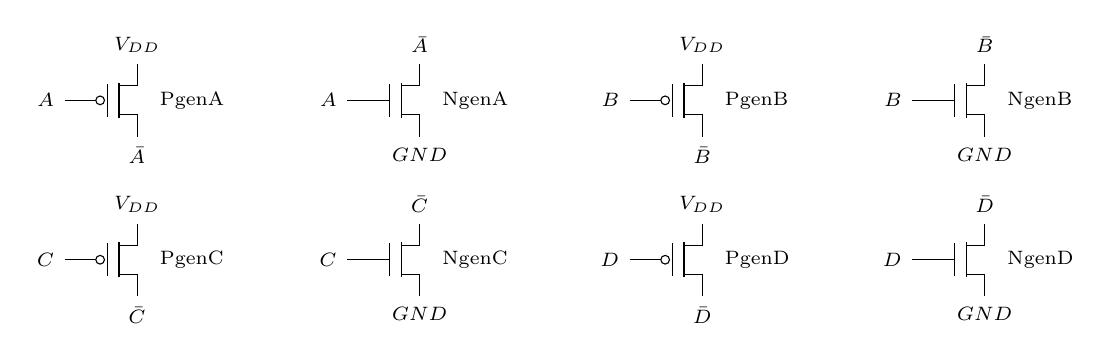
\begin{tikzpicture}[x=.92cm,y=.92cm,font=\scriptsize]
\mos{0.0}{0.0}{A}{1}
\node[right]at(0.43,0.0){$\mathrm{PgenA}$};
\node[above]at(0.25,0.52){$V_{DD}$};
\node[below]at(0.25,-0.52){$\bar A$};
\mos{3.9}{0.0}{A}{0}
\node[right]at(4.33,0.0){$\mathrm{NgenA}$};
\node[above]at(4.15,0.52){$\bar A$};
\node[below]at(4.15,-0.52){$GND$};
\mos{7.8}{0.0}{B}{1}
\node[right]at(8.23,0.0){$\mathrm{PgenB}$};
\node[above]at(8.05,0.52){$V_{DD}$};
\node[below]at(8.05,-0.52){$\bar B$};
\mos{11.7}{0.0}{B}{0}
\node[right]at(12.129999999999999,0.0){$\mathrm{NgenB}$};
\node[above]at(11.95,0.52){$\bar B$};
\node[below]at(11.95,-0.52){$GND$};
\mos{0.0}{-2.2}{C}{1}
\node[right]at(0.43,-2.2){$\mathrm{PgenC}$};
\node[above]at(0.25,-1.6800000000000002){$V_{DD}$};
\node[below]at(0.25,-2.72){$\bar C$};
\mos{3.9}{-2.2}{C}{0}
\node[right]at(4.33,-2.2){$\mathrm{NgenC}$};
\node[above]at(4.15,-1.6800000000000002){$\bar C$};
\node[below]at(4.15,-2.72){$GND$};
\mos{7.8}{-2.2}{D}{1}
\node[right]at(8.23,-2.2){$\mathrm{PgenD}$};
\node[above]at(8.05,-1.6800000000000002){$V_{DD}$};
\node[below]at(8.05,-2.72){$\bar D$};
\mos{11.7}{-2.2}{D}{0}
\node[right]at(12.129999999999999,-2.2){$\mathrm{NgenD}$};
\node[above]at(11.95,-1.6800000000000002){$\bar D$};
\node[below]at(11.95,-2.72){$GND$};
\end{tikzpicture}\end{center}
With these generators, the fully differential design uses 18 MOS and DSL uses 20. The dynamic circuit needs only the original inputs and uses six. Repeated names in every drawing denote electrically connected terminals.
\newpage
\section*{Question 8: conceptual answers}
\begin{enumerate}[label=(\alph*),leftmargin=*]
\item \textbf{Latchup:} lower well/substrate resistance with frequent low-resistance body taps; add correctly biased guard rings to collect injected minority carriers and reduce the parasitic bipolar feedback. A latchup-resistant process is another valid approach. These interrupt the parasitic pnp/npn regenerative path.
\item \textbf{Standard-cell layout:} use the library's fixed row height and aligned power/ground rails so neighboring cells abut; obey the library's placement/routing grid, boundary rules and accessible pin locations so abutment and routing remain legal. Cell widths may vary on the permitted site grid.
\item \textbf{Soft-error masking:} logical masking blocks a transient when a gate's other inputs are controlling; shallower pipeline logic can provide fewer blocking opportunities, but logical masking depends on the function and input pattern, not scaling alone. Electrical masking attenuates a narrow/weak pulse below the next gate's effective threshold; smaller capacitance and critical charge, changed restoring currents and gate delays can make smaller particle-induced pulses harmful. The effect is technology dependent, so scaling does not universally eliminate electrical masking. Latch-window masking occurs when a surviving pulse misses the sampling aperture. For a random arrival phase, a simplified capture fraction scales like $\min[1,(w_{pulse}+t_{setup}+t_{hold})/T]$; reducing T increases capture opportunities. More vulnerable nodes and smaller critical charge further affect chip-level SER. A universal numeric SER does not follow from frequency alone.
\item \textbf{Supply/ground bounce:} reduce shared package/bond-wire inductance with more and shorter parallel supply/ground connections; reduce simultaneous $di/dt$ with controlled-slew/staged IO drivers or staggered switching. Both reduce the inductive disturbance $\Delta V\simeq L\,di/dt$.
\item \textbf{Dynamic logic:} charge sharing can lower a precharged rail without a complete discharge path; direct cascades of ordinary same-phase dynamic gates can evaluate incorrectly while an upstream rail is still precharged. Leakage/retention is another genuine issue, addressed in Q3.
\item \textbf{Domino limitations:} the usual n-domino structure realizes only noninverting functions at its buffered output; each stage needs a restoring output buffer, with inputs respecting evaluation monotonicity. The buffer adds area/capacitance and constrains structure.
\item \textbf{Core-limited:} required logic/memory area sets die dimensions, with pads fitting around the core. \textbf{Pad-limited:} the number and pitch of peripheral IO pads set a larger die perimeter than the core alone requires.
\end{enumerate}

\textbf{Primary conceptual references.} \href{https://www.ee.ncu.edu.tw/jfli/public_html/VLSI/lecture/ch03.pdf}{Li, Chapter 3, slides 31--36} supports latchup mechanisms and guard rings. \href{https://www.ee.ncu.edu.tw/jfli/public_html/VLSI/lecture/ch06.pdf}{Chapter 6, slides 13--18 and 29--33} supports dynamic/domino limitations and differential/DSL structures. \href{https://users.cs.utah.edu/~rajeev/cs7810/papers/shivakumar02.pdf}{Shivakumar et al., DSN 2002} analyzes electrical and latching-window masking trends; the explanation above distinguishes those trends from a universal scaling claim.

\textbf{Verification and limits.} Run \texttt{python verify.py}. It verifies the RC/sizing families, clock gate capacitance, literal layout graph and its source anomaly, all eight sequential input words and structural paths, signed-skew setup/hold, 243 resistor-divider cases, and sixteen complementary-network inputs. These are analytical/conduction checks. No HSPICE result, private process model, or unprovided device strength is claimed.
\end{document}
